
% Package for including code in the document
%\usepackage{listings}


The first part of the assignment was 
\begin{quote}
	You are given a total of 150 four dimensional samples of three Iris species.  Use Multiple Discriminant Analysis (MDA) to separate the samples into three Iris species. Show the resulting misclassifications.   Repeat MDA choosing any three-dimensional features at a time and show the resulting misclassifications.
\end{quote}

The Mathematica version is long mostly from listing the samples.  Other than that, the steps mimic the algorithm for MDA very closely.  Once the structure allows for a classifier to is constructed on the assumption that the data is Gaussian.  

\begin{lstlisting}{language=Mathematica}
barSetosa = Mean[setosa]
barSetosaArray = PadLeft[{barSetosa}, First[Dimensions[setosa]], {barSetosa}]
normSetosa = setosa - barSetosaArray
ScatterSetosa = Transpose[normSetosa].normSetosa/First[Dimensions[setosa]]

barVersicolor = Mean[versicolor]
barVersicolorArray = PadLeft[{barVersicolor}, First[Dimensions[
  versicolor]], {barVersicolor}]

normVersicolor = versicolor - barVersicolorArray
ScatterVeriscolor =
         Transpose[normVersicolor].normVersicolor/First[Dimensions[versicolor]\
]

barVirginica = Mean[virginica]
barVirginicaArray = PadLeft[{barVirginica}, First[Dimensions[virginica]], \
{barVirginica}]
normVirginica = virginica - barVirginicaArray
ScatterVirginica = \
Transpose[normVirginica].normVirginica/First[Dimensions[virginica]]
whiteningScatter = ScatterVirginica + ScatterSetosa + ScatterVeriscolor
flowers = Join[setosa, versicolor, virginica]
combinedMean = Mean[flowers]
flowers = Join[setosa, versicolor, virginica]
combinedMean = Mean[flowers]
meanArray = Join[{barSetosa}, {barVersicolor}, {barVirginica}]
combineMeanArray = PadLeft[{combinedMean}, Dimensions[meanArray], \
{combinedMean}]
meanDifference = (meanArray - combineMeanArray)
scatterBackground = Transpose[meanDifference] .(50*meanDifference)
{lambda, W} = Eigensystem [{scatterBackground, whiteningScatter}, 2]
ListPlot[flowers.Transpose[W]]
\end{lstlisting}

\subsection{Explanation of the Mathematica Code}
In the Mathematica example, we use setosa, viriginica, and versicolor as variables containing the original measurements.  We next construct an row matrix contain at each of its rows, called barSetosaArray.  This array is used to generate $\vec{x_i} - \mu$ for row vector $\vec{x_i}$ in the setosa collection, misnomered as normSetosa.  This allows mean to generate the scatter matrix for setosa.  

The same thing was done for versicolor and virginica.  As stated in the MDA algorithm, $\mathbf{S_w} \sum_i S_i$ where $S_i$ are the scatter matrices for each of the classes.  Here also, we combine the flowers using the Join method in Mathematic, and take a mean of the combined whole.  From there, we use the mean array concept to reduce finding the background scatter to matrix addition, scalar multiplication, matrix multiplication and a transpose.  

Fortunately, Mathematica has an intuitive method for computing eigenvectors of a generalized system as below.
\[
\mathbf{A} \vec{e_i} = \lambda_i \mathbf{B} \vec{e_i}
\]
Thus mapping the original data source via the $\mathbf{W}$ obtained is simply a matter of matrix multiplication

\subsection{Plot Results from Mathematica}
\begin{figure}[htbp] %  figure placement: here, top, bottom, or page
   \centering
   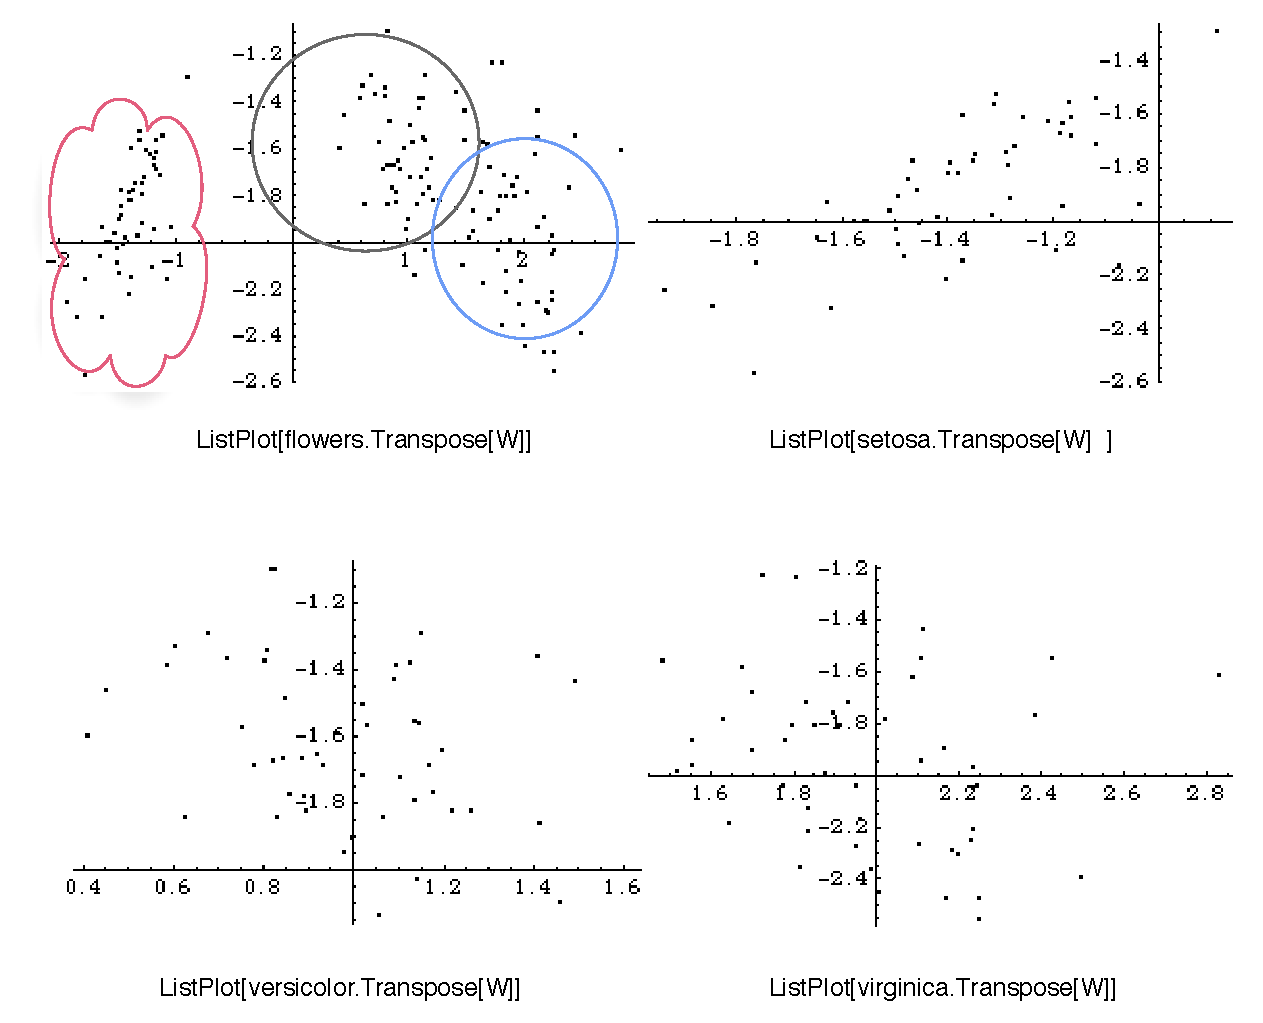
\includegraphics[width=5in]{flowersMDA.pdf} 
   \caption{mathematica Plots using a manual MDA}
   \label{mathematicaPlotsUsingManualMDA}
\end{figure}
